\documentclass[letterpaper]{article}

\usepackage{aaai}
\usepackage{times}
\usepackage{helvet}
\usepackage{courier}

\usepackage{graphicx}
\graphicspath{ {images/} }
\usepackage{enumitem}
\usepackage{color}
\usepackage{subfigure}
\usepackage{hyperref}
\usepackage{dcolumn}

\frenchspacing
\setlength{\pdfpagewidth}{8.5in}
\setlength{\pdfpageheight}{11in}

\pdfinfo{
Forever Blowing Blockchains: Determinants and Dynamics of Speculative Bubbles
/Nicolas Della Penna, Eaman Jahani, Peter Krafft, Octavio Bunge, Harper Reed, Alex "Sandy" Pentland, Julain McAuley}
\setcounter{secnumdepth}{0}  

\begin{document}
% The file aaai.sty is the style file for AAAI Press 
% proceedings, working notes, and technical reports.
%
\title{Forever Blowing Blockchains: Determinants and Dynamics of Speculative Bubbles}
\author{
% 1st. author
Nicolas Della Penna \thanks{indicates equal contributions.}\\
%Nicolas Della Penna \titlenote{is a first co-author of this paper.}\\% He conceived the study, methodology, and wrote the initial manuscript and the notebook with the data analysis.}\\
ANU \\
n@nikete.com
% 2nd. author
\And
Eaman Jahani \footnotemark[1] \\
%Eaman Jahani \titlenote{is a first co-author of this paper.}\\% He wrote the forum scrapers, constructed networks and their measures, and wrote up the relevant sections in network data and variables, wrote the analysis pipeline, helped with definition of coin metrics, and contributed to the writing of the whole paper.}
MIT \\
eaman@mit.edu
% 3rd. author
\And
Peter Krafft \\%\titlenote{helped with methodology and literature review} \\
MIT \\
pkrafft@mit.edu
\And
Octavio Bunge \\%\titlenote{ wrote scrapers for coin prices, and the non-trivialness measure.}\\
Universidad de Belgrano \\
octavio.bunge@\\comunidad.ub.edu.ar
% 4th. author
\AND
Harper Reed \\%\titlenote{helped with the writing and literature review}\\
\\
harper@nata2.org
% 5th. author
\And  % use '\and' if you need 'another row' of author names
Alex (Sandy) Pentland \\ %\titlenote{helped with methodology and writing}\\
MIT Media Lab \\
pentland@mit.edu
% 4th. author
\And
Julian McAuley \\%\titlenote{helped with methodology and writing}\\
UC San Diego \\
jmcauley@cse.ucsd.edu
}
\maketitle


\begin{abstract}
We study the power of structural features of the social network around cryptocurrencies to understand the severity and magnitude of bubbles. We introduce a novel dataset that combines measures of the social network surrounding the introduction of coins in online cryptocurrency forums and the trading behavior across marketplace. Our networks are constructed based on the intensity of social interactions in the main discussion forum of cryptocurrencies. All the structural features of the network are measured based on the state of the social network before the relevant cryptocurrency is ever traded; therefore avoiding any possible confounding between the prices of the assets and community attention.
We find that timing of coin introduction is crucial for bubbles to form.

\end{abstract}

\section{Introduction}
\section{Introduction}

Speculative bubbles are perceived to periodically take over markets \cite{garber2001famous}.
Going back at least to the \emph{South Sea} bubble in the early 18$^{\text{th}}$ century, well-informed parties  have invested knowingly in bubbles, and found it profitable \cite{temin2004riding}.
Today, the public notoriety of Bitcoin, together with its massive price increases and their associated publicity lead to an explosion of attempts to create ``the next Bitcoin''.
Collectively, these currencies are often referred to as ``cryptocurrencies'' or simply ``coins'', and a vibrant set of exchanges have emerged where these are traded, either for each other or money.
The majority of these coins have no possible future valuable in the long term, and their markets would appear to be driven largely by speculation.
Many of them appear to be nothing but attempts at turning a quick profit from inflating the implied valuation of a coin shortly after creating it.
This is driven by the extremely low cost and effort required to create a new coin, with most being minimal changes to parameters and branding of a pre-existing codebase.

Those who make and trade these coins communicate largely online, and much of their activity is concentrated on public forums. 
As such, price and volume data from these exchanges is freely available and widely aggregated\footnote{ these are however largely unregulated, often anonymous, and there is no way to account how much of reported volumes are manipulation attempts. The existence of attempts at arbitrage between them places some bounds on how blatantly the data can be manipulated for prices, but volumes are impossible to assess. },
%JULIAN: Whole footnote is one extra-long sentence!
and the source code to all of them being public is the norm%\footnote{cargo cult CS being derigour in the comunity}.
This makes cryptocoins
%JULIAN: cryptocoins is a new work--maybe avoid mixing the terms
an ideal lens through which to study the social life of a ``market mania'' \cite{cosma2008}.
Such a study is valuable both as a means of understanding the dynamics of bubbles themselves, but also from a computational social science perspective, to understand the ecosystem and lifecycles of these online communities.
%Such a study can serve in the computational social sciences a role analogous to that of lesion studies do in neuropsychology.
%JULIAN: Not obvious to me what the above analogy is without further explanation.


%\begin{figure}[h!]
%\end{figure}

We present a study of a large number of cryptocurrency ecosystems, 
using a novel dataset that combines measures derived from social networks of users in cryptocurrency forums, market data aggregated over dozens of exchanges, and properties of the software implementing the cryptocurrencies themselves.
From forums we identify the introducers of each coin and build measures of their position in the network based on
%which users have engaged with them
their patterns of engagement in forum threads
%threads in the forum
\emph{before} the coin is announced.
In this way we identify 376 coins that are announced by users of the forum and which can be mapped to price and volume data from exchanges.
Next, from price and transaction volume data we build measures of the subsequent activity that results from trading in the coin. 
We also assess if coins possibly embody technological innovation based on having more than trivial modifications to previously existing coins' source code.


%\begin{figure}
%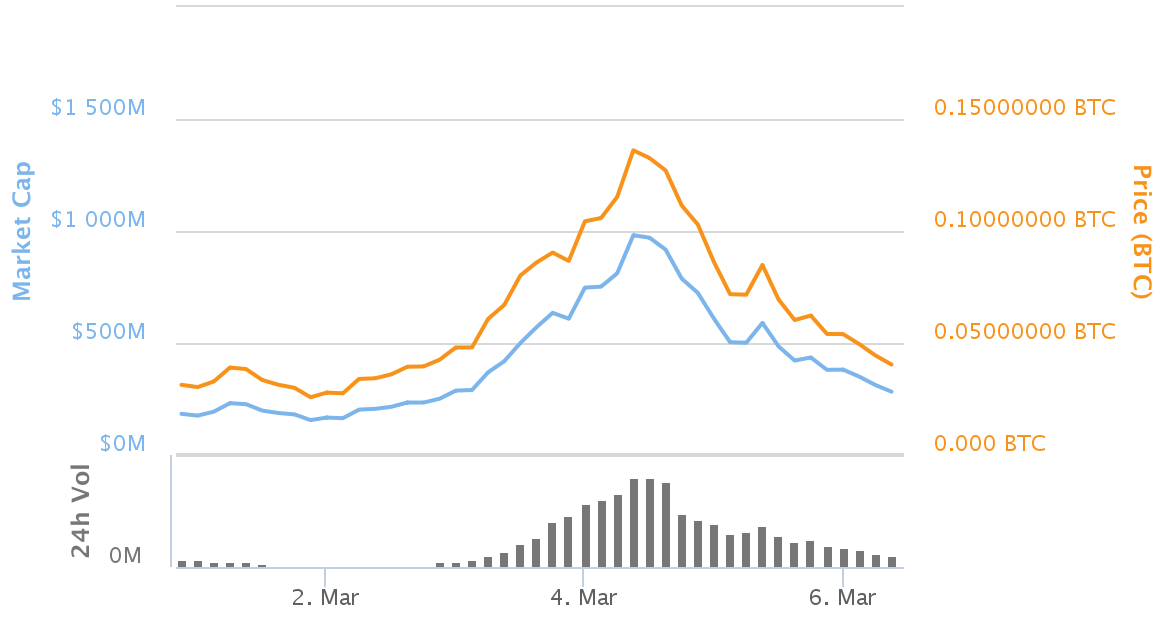
\includegraphics[width=\columnwidth]{AuroraCoin}
%\end{figure}

While the mechanisms that drive bubbles have been studied both theoretically 
\cite{abolafia1988enacting, earl2007decision, bakker2010social, harras2011grow}
and experimentally
\cite{moinas2013bubble},
% in the lab, 
an exhaustive dataset and study of the social networks of those promoting the asset has not been previously previously possible.
While the magnitude of the assets traded is certainly small relative to most financial and commodity markets, it is nevertheless much larger than
%JULIAN: Found this sentence a bit funny, not that I could improve upon it
even the most lavishly funded experimenter could hope for.
For example, the largest bubble in our dataset, AuroraCoin, reaches a valuation of one billion USD in March 2014,
with reported daily trading volumes of 6.8M USD, and sheds 90\% of its value in a week, and 99\% of its value in well under a year.
For context, this is equivalent to one quarter of Iceland's entire foreign exchange reserves in 2014,\footnote{4.1 Billon USD, The World Bank, Global Economic Monitor, accessed October 2015} the population of which AuroraCoin promoters claimed they would distribute half of the coins to.

\begin{figure}
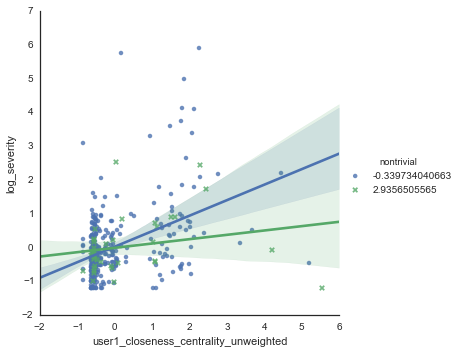
\includegraphics[width=\columnwidth]{severity_centrality}
\end{figure}

Using price and volume data we construct measures of both the magnitude and the severity of bubbles.
These are defined formally in our variable section,
%JULIAN: Give a section ref?
but their intuition is that we say the magnitude of a coin is large when a high volume in dollars of trades happens,
%JULIAN: Does it make a difference what it's measured in?
while we say a coin has a severe bubble if investing a fixed amount leads to loosing a large proportion. 
By considering the community structure that exists in the forum before a coin is introduced we are able to predict a substantial fraction of the variation in both the severity and magnitude of the resulting bubble.
This is a challenging task, and models that rely on either simple activity or network metrics metrics show almost no predictive out-of-sample power, unable to explain even 1\% of the variation in either task,
our best models perform an order of magnitude better in both tasks.
%JULIAN: R^2 of 0.1 (if I interpret correctly) doesn't sound impressive until you've argued the fundamental difficulty of the problem, you might wait to mention such numbers.
%JULIAN: Would sound more impressive if you just said "it performs an order of magnitude better"
The main driver of our explanatory power is the centrality of a user in the directed network derived from the forum. 
This effect appears to be mediated by whether a coin involves a nontrivial technological change, the direction of the interaction reversing depending on whether it relates to magnitude or severity.
%JULIAN: Above sentence is tough to parse, but kind of an important one.
Both the severity and the magnitude of bubbles increases with the centrality of the user who introduces the coins in the forums.  
Interestingly this effect is concentrated in different ways depending on whether the coin software is more than a trivial modification: trivial coins have more severe bubbles the more central their introducers are, while volume is greater the more central the introducer of a nontrivial coin is.




%JULIAN: Needs something outlining the paper's main results here, ideally a figure explaining the role of the various parts of the system.
%JULIAN: I'd tone down the footnotes

\begin{figure}
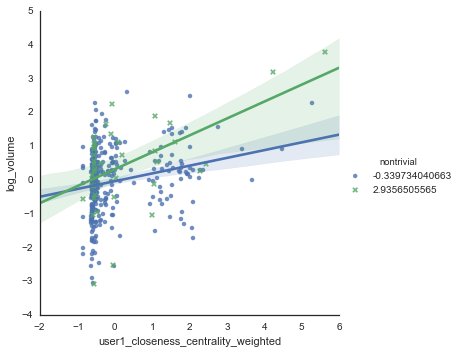
\includegraphics[width=\columnwidth]{volume_centrality}
\end{figure}

%Methodologically the free parameters in the way we do the weights on the weighted graph  is horrible, a million free parameters get introduced. follow up work for another paper: do some unsupervised feature learning over the dam forums threads to build the network; use some internal validity metric . Find political way of saying this in future work.
\section{Literature}
\section{Lit}

Agents structural strength within the discourse surrounding cryptographic currencies is particularly important, as these are almost entirely performative; the initial marketplace adoption of bitcoin is 
crash of  %87 http://www.iijournals.com/doi/abs/10.3905/jpm.1989.409242?journalCode=jpm 
“rapid rise of options” with the rise of the theory to price those options, in having currencies with zero entire costs
MacKenzie, Donald. "An Engine, Not a Camera."
While states can create the demand required for a currency system to run by compelling tax payment in it (for a recent example), non state sponsored currencies must find some other ways of creating demand.
The initial market for which bitcoin has been used (prices denominated in it, transactions only in it) where drug sales. citation.
New currencies have thus been floated with every single drug name possible. Many chains can claim to the same claim, so exchanges (since speculation is the only possible use of almost all of them) become de-facto stabilizers of who has a minimally viable claim. 









Network Diversity and Economic Development
http://www.sciencemag.org/content/328/5981/1029.full



"Hence, highly clustered, or insular, social ties are predicted to limit access to social and economic prospects from outside the social group, whereas heterogeneous social ties may generate these opportunities from a range of diverse contacts (1, 2)."

"Although both social and spatial network diversity scores were strongly correlated with IMD rank, we found a weaker positive correlation present using number of contacts and a negative correlation for communication volume."

"For example, whereas inhabitants of Stoke-on-Trent, one of the least prosperous regions in the UK, averaged a higher monthly call volume than the national average, they have one of the lowest diversity scores in the country. Similarly prosperous Stratford-upon-Avon has inhabitants with extremely diverse networks, despite no more communication than the national average. "




Predicting Spending Behavior Using Socio-mobile Features:
http://ieeexplore.ieee.org/xpl/login.jsp?tp=&arnumber=6693330&url=http%3A%2F%2Fieeexplore.ieee.org%2Fxpls%2Fabs_all.jsp%3Farnumber%3D6693330
free version:
https://scholar.google.com/citations?view_op=view_citation&hl=en&user=Ef1hJ8IAAAAJ&sortby=pubdate&citation_for_view=Ef1hJ8IAAAAJ:NaGl4SEjCO4C

Social behavior can be used to predict spending behavior in couples in regards to their prepensity to diversify the businesses they explore, become loyal customers and overspend. The results show that mobile phone social interaction patters can be more predictive than personality based features when predicting spending behavior. 

"We find that social behavior measured via face-to-face interaction, call, and SMS logs, can be used to predict the spending behavior for couples in terms of their propensity to explore diverse businesses, become loyal customers, and overspend"

"results show that mobile phone based social interaction patterns can provide more predictive power on spending behavior than personality based features. Interestingly, we find that more social couples also tend to overspend."




Money Walks: Implicit Mobility Behavior and Financial Well-Being:
http://journals.plos.org/plosone/article?id=10.1371/journal.pone.0136628

Spatiotemporal traits such as exploration, engagement and elasticity can be used to predict future finanical difficulties. 

"Hence, in this work we study a large-scale cross-sectional dataset of human spending across space and time, and connect it to the biological phenomena of “foraging,” a basic pattern of animal movement to gather foods and resources."

"we analyzed a corpus of hundreds of thousands of human economic transactions and found that financial outcomes for individuals are intricately linked with their spatiotemporal traits like exploration, engagement, and elasticity. Such features yield models that are 30\% to 49\% better at predicting future financial difficulties than the comparable demographic models."

"As shown in Fig 2, individuals with lower levels of education (High School, Middle School, or Primary School) were found to be more likely to be late for their payments and get into financial trouble. Users with higher age were marginally less likely to overspend, miss payments, or get into financial trouble. Last, male customers and married customers were less likely to miss their payments."

"The figure also shows that multiple mobility behavior features were statistically correlated with outcome variables, even after controlling for the effect of abovementioned demographic variables of age, gender, marital status, education, and work type."

"the behavioral features were found to be more significantly associated (in terms of p-values) and contain higher predictive power (in terms of odds ratios being further away from 1.0 in either direction) as compared to the demographic features."

"The evidence so far indicating that each of the spatio-temporal behavioral descriptors has significant association with different financial outcomes motivates their combination to predict the financial outcome"




Predicting personality using novel mobile phone-based metrics
http://dl.acm.org/citation.cfm?id=2456492
free version:
https://www.google.com/url?sa=t&rct=j&q=&esrc=s&source=web&cd=1&ved=0CCEQFjAAahUKEwivqbnj0L3IAhWIcT4KHZtqCOg&url=http%3A%2F%2Frealitycommons.media.mit.edu%2Fdownload.php%3Ffile%3DdeMontjoye2013predicting-citation.pdf&usg=AFQjCNGDDMiemMv9vPQGBd_NNP30sEr6MQ&sig2=CQk3pVIzJ3EmXlV0lD8oKA

"Using a set of novel psychology-informed indicators that can be computed from data available to all carriers, we were able to predict users’ personality with a mean accuracy across traits of 42% better than random, reaching up to 61% accuracy on a three-class problem."

"The goal of the present research is to show that users’ personalities can be reliably inferred from basic information accessible from all mobile phones and to all service providers."

"The model predicted whether phone users were low, average, or high in neuroticism, extraversion, conscientiousness, agreeableness, and openness with an accuracy of 54%, 61%, 51%, 51%, and 49%, respectively."




\section{Data Description}
\subsection{Prices, Exchanges, and Coin characteristics}
\begin{figure}[h]
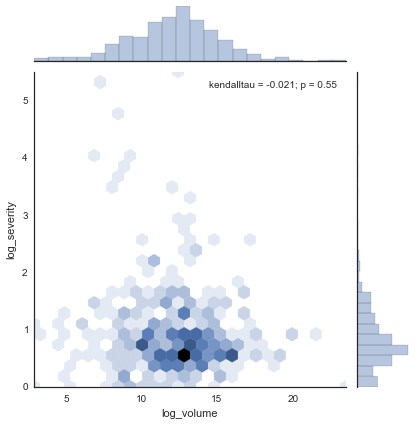
\includegraphics[width=\columnwidth]{severity_volume}
\end{figure}

Our main outcome measures are the severity of drop in the value of a unit of the asset, and the magnitude in USD of the transactions in it.
We scrape daily price and volume data from coinmarketcap.com\footnote{ For robustness analysis smaller subsets of the coins where available from coin }
%JULIAN: Didn't follow the above footnote
We operationalize the severity of a bubble as the inverse of 1 dollar that would be lost buying at the maximum price and selling after that proportionally to the volume of the market until the present; we call this severity.
%JUliAN: Above is hard to follow if not spelled out in the form of equations; wordy papers with everything explained inline seems more economics and less WWW
We define the volume as the sum of the dollar volume of trade reported over all exchanges.

\subsection{Nontrivial coins}

Many of the coins available in the exchanges are trivial modifications of another coin in that they only change parameters such as the name, the number of total mineable coins, or the transaction time between blocks.
These coins' production cost is virtually zero\footnote{ there is a cottage industry that offers the creation of binaries and provisioning of mining and bandwidth as a bundled service that require no technical skill to create form the user, examples are Coingen or Coincreator}.

To attempt to capture this we analyze data from mapofcoins.com which includes a genealogy of coins and data from the github page of coins not available on mapofcoins.com.
If the coin to be analyzed has a parent and the algorithm it uses differs from the parent or if it has no parent, it is labeled as nontrivial, meaning that the coin implemented something that did not previously exist, and is not just a fork with only parameters changed, such as total mineable coins, transaction speed, etc.


\subsection{Forum Discussions}
In order to study the effect of communication networks around cryptocoins on
price variations, we collected all the posts from the most popular cryptocurrency
online community, \url{https://bitcointalk.org}.  Our data consists of all the posts that were
made between January 2010 and July 2015 on the most active crypto-related forums:
\begin{enumerate}[topsep=0pt,itemsep=-0.5ex,partopsep=1ex,parsep=1ex]
  \item \textbf{Bitcoin Discussion:} This is the oldest forum on the website which mainly focuses
    on issues related only to Bitcoin. Interestingly, Satoshi Nakamoto, the alleged
    creator of Bitcoin made the first post on this forum in January 2010 and
    was active until January 2011. The presence of Satoshi in the data set enables us
    to study the position of various actors in the online community relative to Satoshi
    and its relation with the success or failure of cryptocoins they advocate or reject.
    %JULIAN: Why is people's relationship to Satoshi likely to be interesting or important?
  \item \textbf{Altcoin Discussion:} This is the most active forum in the community
    with more than 730,000 posts as of July 2015, dating back to June 2011.
    The discussions in this forum mainly evolve around alternative currencies
    other than Bitcoin. Users often discuss the merits or flaws of various
    altcoins or simply exchange technical information.
  \item \textbf{Announcement (Altcoin):} Community announcements such as development of 
    exchange clients or addition of new features are made here. This is an important forum
    in our study as the creation of new altcoins are announced here. Whenever a new
    altcoin is announced to the community, the announcement is tagged with string ANN.
    This enables us to detect announcements of new coins into the market and identify
    the users who introduced them for the first time.
  \item \textbf{Mining (Altcoin):} Technical issues pertaining to mining (i.e.~validating transactions)
    altcoins are discussed here.
  \item \textbf{Marketplace (Altcoin):} This forum contains the discussions on a wide-range of 
    market-related issues, such as price or volume trends, possible pump-and-dump schemes
    and exchange tips.
\end{enumerate}

Each forum consists of many subjects or threads initiated by different users.
Each thread contains several posts or replies, with an average of 10 posts per
thread.  The reply structure within each thread constitutes the basis of our
forum network, discussed below.  Each post has several fields which contain
valuable information in our context.
\begin{enumerate}[topsep=0pt,itemsep=-0.5ex,partopsep=1ex,parsep=1ex]
  \item \textbf{Subject:} Usually, the initiator of the thread chooses subject and all the
    following posts inherit the same subject.
  \item \textbf{Content:} The actual text of the post.
  \item \textbf{Position in the thread}: The later posts in the thread might not be as important
    as earlier posts and could be about issues other than the original topic of the thread.
  \item \textbf{Author}
  \item \textbf{Date}
\end{enumerate}
The community had only 10,000 unique users until early 2013, however it grew considerably faster after 2013 and reached about 70,000 by early 2015.
Nevertheless, there are only around 10,000 active users within any 30 day period on average.
Figure \ref{aurora_thread} shows an example of the first post in a thread which introduced Aurora coin for the first time in the Announcement forum.

\begin{figure}

\includegraphics[width=0.99\columnwidth]{aurora_thread_cut.pdf}
\caption{The first post of a thread announcing the release of Auroracoin for the first time in \url{https://bitcointalk.org} 
\label{aurora_thread}
\end{figure}

%JULIAN: Being crass, just showing a quick figure with an example of a discussion wouldn't hurt. I have no idea what people discuss on forums like this, so a figure whose purpose is to convince me that there's meaningful signal here could be helpful


\subsection{Forum Interaction Network}

Given the forum discussion data at the level of individual posts, we  construct a network capturing the discussion patterns among users. The structural properties of this network form the basis of our analysis on a per-coin basis. In this network, nodes are the forum users and \textit{directed edges} point from posters within each thread to thread-initiators. The omission of edges based on simple co-appearance within a thread leads to a sparser network which isolates the communication patterns around ``dialogue-shapers''. The edges in the discussion network are weighted by the number of times a poster replies to a thread-initiator in different threads (i.e.~multiple replies by the same user within the same thread are counted only once).
% Is this too big of a statement?
In this context, edge weights capture the level of engagement thread initiators receive from the community and the amount of information a poster receives from thread initiators. Furthermore, our network construction method uses all the interactions since the inception of bitcointalk in creating new edges or updating their weights. The unlimited retention of any such (replier to thread initiator) interaction captures relevant information on seniority and community influence which are obtained through long-term and persistent presence in the forums. 

%Prior to construction of the network, we merged posts from all forums into a
%single large forum since the community base of all five forums mentioned
%above is made of the same users and we are mostly concerned about influence and
%aggregate information flow among users, rather than the exact topic of the discussion.
To build our network, we first combine the posts from all forums. We do this because the community base of all five forums mentioned above is made of the same users, and because we are mostly concerned about influence and aggregate information flow among users, rather than the exact topic of the discussion.
The network construction involves replaying all the posts over time sorted by their date and updating the
discussion network accordingly. Whenever a new altcoin is introduced
in the forum for the first time, the user who introduced it and a snapshot of the network is taken. 
We analyze the discussion network only up to the first time each coin is introduced to the community, in order to avoid any possible confounding between a coin's price movement and the extra attention it receives in the community due the same price changes. Our method uses the position of the first introducer in the network snapshot and the general structure of her neighborhood for extracting various network measures corresponding to that coin. Our final analysis examines these per-coin measures for evaluating the performance of each coin.



%TODO Do we use the date of the ANN or the date of the first trade?!?! NIKETE & EAMAN.
% E: Both of them are in the file, depends which one you are using. 
%The identification of true introductions of new altcoins is a difficult process prone to many false-positives. 
The  majority of such introductions are made in the \textit{Announcement} forum and are preceded with the ``ANN'' tag. We look for the first mention of both the coin symbol \textbf{and} its descriptive name in the subject of a thread which contains the announcement tag. \textcolor{red}{The first mentions of either the coin symbol \textbf{or} its name are used as a fall-back in case the more restrictive \textbf{and} requirement did not detect the first introduction of the coin.}
%JULIAN: The above seems like a long winded way of saying that you just used "or". i.e., the above sentence parses to "(a and b) or (a or b)". Didn't want to overwrite in case I misunderstood.
% EAMAN: remove the text on OR requirement, if you did not or do not plan on falling back on OR mentions.
Using the more restrictive matching requiring both the coin name \textbf{and} symbol be present in the subject, we are able to detect the first introduction of 376 altcoins out of 679. \textcolor{red}{We can detect an extra 176 altcoins by falling back on the \textbf{or} requirement.}
% Eaman: remove text in red if not falling back on OR.
The forum user who initiated such a thread is assigned as the introducer of the coin to the community.

%TODO(NIKETE): add validation results table wrt mapofcoins data here ?



\section{Variables}
\subsection{Magnitude and Severity}
Our main outcome measures are the severity of the largest drop in the price of each cryptocoin, and the magnitude (volume) of the transactions made with the cryptocoin measured in USD.
We operationalize the intensity of a bubble as the proportion of a 1 dollar that would be lost buying at the maximum price and selling after that proportionally to the volume of the market till the present. Magnitude of a bubble is defined as the proportion of the average daily volume prior to maximum price to the overall average daily volume.
More formally for each coin $c$, let $P_c,V_c$ be two vectors of length $T$ each indexed by days since the coin $c$ started trading.
Let $v_{c,t}$, the $t^{th}$ element of $V_c$ be the number of $c$ coins traded across all exchanges $t$ days after $c$'s introduction to the market. 
Similarly, let $p_t$ be the representative price of coin $c$ on day $t$ \textcolor{red}{measured in USD}.
\footnote{There are several ways that this can be defined reasonably. For the markets organized as continuous double auctions the price of the first or last transaction of the day,  the average price transacted during a day, the average best asking bid at midnight or noon, would all be reasonable choices. Exchange price aggregators and exchanges own historical data do not provide enough precision to pin this down, as it is entirely possible that the aggregators are using inconsistent definitions for the underlying exchanges.}. Then, we simply define our magnitude measure for coin $c$ as
\begin{equation}
magnitude_{c} = \frac{\sum_{t=1}^{t_{max}} v_t p_t} {\sum_{t=1}^{T} v_t  p_t} \frac{T}{t_{max}}
\end{equation}
where $t_{max}$ is the date in which the coin realized its maximum price and T is the number of days since the introduction of coin $c$ to the market until present ($t_{max} < T$). Note that the magnitude is normalized by the length of time coin has been present in the market.

Similarly, the average price after $t_{max}$ weighted by daily volume is defined as:
\begin{equation}
\bar{p}_{t_{max},T} = \frac{\sum_{t=t_{max}}^{T} v_t p_t} {\sum_{t=t_{max}}^{T} v_t}
\end{equation}

We define the severity of the bubble experienced by the coin $c$ as the fraction of the maximum price lost relative to average price since $t_{max}$ until present:
\begin{equation}
severity_{c} = \log(\frac{ p_{t_{max}}} {\bar{p}_{(t_{max},T)} })
\end{equation}

Figure \ref{log_magnitude_log_severity} shows the distribution of our constructed dependent variables and their relationship. Both of the variable exhibit a heavy-tailed distribution which makes it necessary to use a robust regression method.

\begin{figure}
\centering
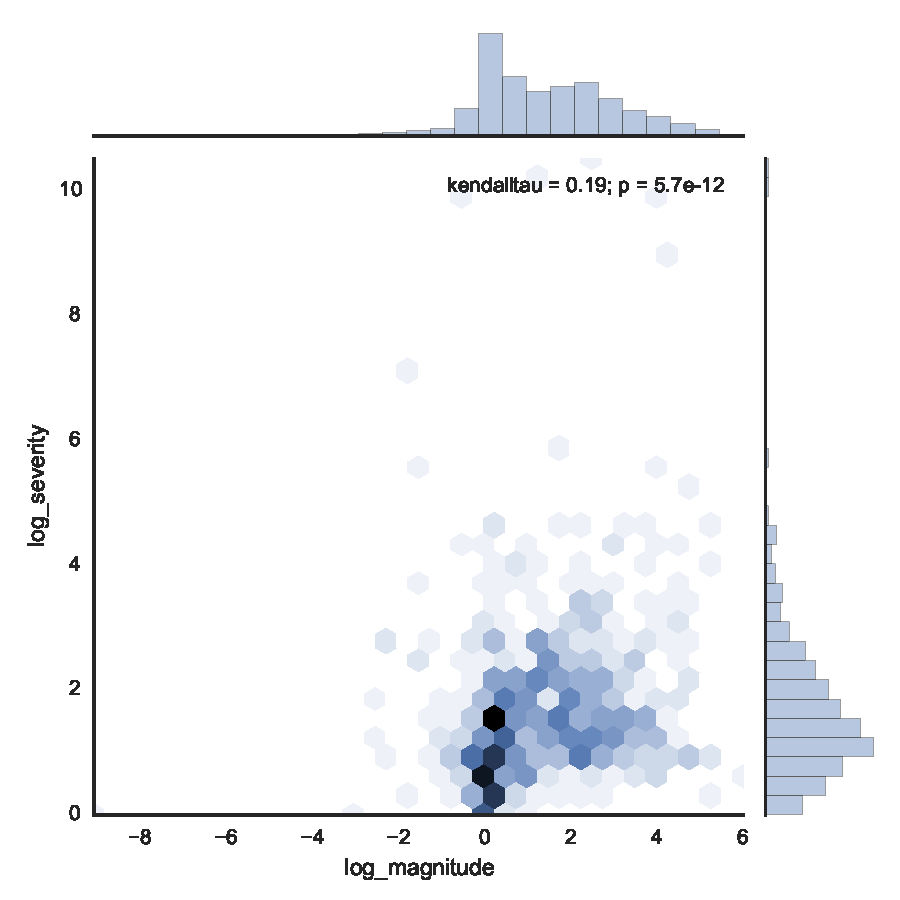
\includegraphics[width=\columnwidth]{log_magnitude_log_severity.pdf}
\caption{The relative distribution of our dependent variables. Note that the magnitude is shown in terms of its natural log due to its heavy-tailed distribution. Both outcome measures exhibit a heavy-tailed non-normal distribution which is a violation of simple OLS assumptions. For this reason, our analysis uses a robust regression method using Huber weights.}
\label{log_magnitude_log_severity}
\end{figure}

\subsection{Network Structure}
\subsection{Network Structure}
In this section, we discuss the various metrics extracted from discussion networks and used as independent variables in the regression analysis. Many of these variables are standard metrics in graph theory designed to capture node centrality is specific scenarios \cite{KleinbergNetworks}. As mentioned before, each coin is associated with a forum user and a discussion network which corresponds to the state of the forum at the time the user introduced the coin to the community. All of our node-level variables refer to the user introducing the coin. Below, we list the network variables included in the analysis. We used Python igraph implementation for computing the network-related metrics \cite{igraph}.
\begin{enumerate}[topsep=0pt,itemsep=-0.5ex,partopsep=1ex,parsep=1ex]
  \item \textbf{Introducer number of posts:} The total number of posts (thread-initiations or simple replies) the coin introducer has made at the time she introduces the coin. It captures the user's level of activity in the community.
  \item \textbf{Introducer number of threads:} The total number of threads the coin introducer has made. Users who start many threads are more likely to receive incoming edges and to shape the dialogue in the community.
  \item \textbf{Seniority:} It is the number of days since the user's first post in the forums. We use this as a proxy for user's seniority in the community.
  \item \textbf{Incoming degree:} The (incoming) degree centrality captures the role of dialogue-shapers in the community as it is the number of unique users who have replied to any of the focal user's threads.
  \item \textbf{Outgoing degree:} The (outgoing) degree centrality captures the role followers in the community as it is the number of unique thread initiators the focal user has ever replied to. 
  \item \textbf{Total degree:} The (undirected) degree centrality captures the total level of the user's involvement in the community in any of the two forms above.
  \item \textbf{Clustering Coefficient:} A measure of embeddedness or triadic closure, this is the fraction of the focal user's triads that are closed. In general, ideas are more likely to be reinforced and persistent in a triad if it is `tightly-knit'. The positive effect of triadic closure (and balance) on tie qualities and their persistence is shown to exist in online social network such as Twitter \cite{KleinbergBalance}, and we believe the same argument applies to our scenario.
  %JULIAN: To be honest I'd do away with most of the above definitions for the social networks track, and just quickly list the features. A quick explanation of why they ought to be useful would be valuable, but definitions for these basic concepts is overkill.
  \item \textbf{Unweighted closeness centrality:} While degree centrality measures the level of user engagement in the community, it only examines the local structure around the user.  In contrast, closeness centrality measures the level of the user's engagement with the global network \textit{either directly or indirectly}. It is relevant in many scenarios, including in online discussions, as information spreads via shortest paths. 
  
  In our context, a user with high closeness centrality has interacted with a diverse set of users who themselves are close to a large set of diverse users.  Our analysis consisted of three versions of the unweighted closeness centrality:
  \begin{enumerate}
    \item \textbf{Incoming:} Only the directed paths leading to the focal user are used. It measures closeness of the whole network to the focal user. Users who start many threads are likely to have higher incoming closeness centrality.
    \item \textbf{Outgoing:} Only the directed paths starting from the focal user to all the other users are used. It measures closeness of the focal user to the whole network. Users who reply to many threads are likely to have higher outgoing closeness centrality.
    \item \textbf{Undirected:} The paths both from and to the focal users are used. Users who initiate and reply to many threads are likely to have higher undirected closeness centrality.
  \end{list} 
  All measures are normalized by the number of users present in the network at the time of coin introduction, so that the comparison between the closeness centrality of various users (who introduce the coins) at different times  is valid. 
  \item \textbf{Weighted closeness centrality:} Similar to the unweighted closeness centrality above, we computed three different versions, with the exception that edges are weighted to indicate the intensity or level of interaction between the two users. The edge weights in our discussion network are determined by the frequency of interactions between two users; and as two users interact more, they are deemed to be closer in their shortest path. Thus in the computation of weighted closeness centralities, we use the reciprocal of the weights as the distance between two users.
  \begin{equation}
    C_{i} = \frac{N-1}{\sum_{j=1}^{N}\sum_{e \in S_{ij}} \frac{1}{w_{e}}}
  \end{equation}
  where $e$ denotes an edge in $S_{ij}$ the set of users on the shortest path from i to j. $w_e$ is the weight of edge $e$ determined by the number of interactions between the end points.
  
  \item \textbf{Weighted betweenness centrality:} Betweenness is closely related to the theory of weak ties and structural holes and measures how well of a bridge is the focal user. In our context, one could interpret betweenness centrality as a generational bridge. Bitcointalk has been an active forum since early 2010, and many users who were once active in its early days are no longer present in the forum. There are however some early users who are still active on the forum. These users have high betweenness centrality as they act as generational bridges between founders and the newcomers to the community. Another standard interpretation of high betweenness centrality is the existence of users who simulatenously interact with two isolated communities in the forum. Similar to closeness centrality, our betweenness centrality computation uses the inverse of edge weights as the distance between two users.
  \item \textbf{Satoshi distance:} Distance to Satoshi can be interpreted as founder effect. Closeness to or direct interaction with Satoshi constitutes as a form of social capital in the community.
  \item \textbf{Weighted pagerank:} where higher weights measured by the frequency of interactions facilitate the flow.
  \item \textbf{Weighted Satoshi pagerank:} is similar to regular pagerank above with the only difference that resets of the random walk always direct to Satoshi instead of a uniform distribution over all users. It can be interpreted as the level of influence or creditability allocated from the founder to other users.
   
\end{enumerate}


\section{Methods }
% Great explanation on R-squared in weighted least square:
% http://stats.stackexchange.com/questions/83826/is-a-weighted-r2-in-robust-linear-model-meaningful-for-goodness-of-fit-analys

\subsection{Models}
We consider seven models each consisting of a different set of explanatory variables corresponding to different levels of available information.
\begin{enumerate}[topsep=0pt,itemsep=-0.5ex,partopsep=1ex,parsep=1ex]
 \item The baseline model incorporates simple user characteristics that are easily observable from her activity on the forum before the introduction of the coin: the number of posts made, the number of threads initiated, the time since first post on the forums (seniority), the number of unique users responded to (out-degree) and the number of unique users from whom a response is received (in-degree).
 \item The nontrivial model includes a single binary variable which indicates whether the source code of the coin contains actual technological innovation and is not simply a trivial change on current existing coins.
 \item The Satoshi model evaluates the possibility of any founder effect and uses information regarding user's position in the discussion network relative to Satoshi, namely Satoshi distance and Satoshi pagerank.
 \item The network model includes network explanatory variables: user's clustering coefficient, closeness and betweenness centrality and her pagerank. Unlike baseline model, these incorporate network-wide information and require access to the full discussion network.
 \item The interaction model investigates the possibility of interaction between user structural features in the network and coin's nontrivialness. In particular it includes 7 interaction terms between clustering coefficient, closeness centrality, betweenness centrality, pagerank, Satoshi pagerank, incoming degree, outgoing degree and nontrivialness variable.
 \item The user model incorporates all the information that's available about the user either from the whole network structure or through her activity in isolation. In other words, it includes all the variables from baseline, Satoshi and network models above.
 \item The final model (All) includes all the variables (18 total) mentioned in all the models above.
\end{enumerate}


\subsection{Model Fitting}
Before attempting to explore the data or fit any of the models, we set aside 40\% of the data points (\textcolor{red}{222}) as test set to evaluate out final model out-of-sample test error. Initial analysis, parameter tuning and model fitting and selection were conducted using the remaining 60\% of the data points (\textcolor{red}{331}). The coefficients and their significance are derived using the train data.

We employed the following procedure for fitting any of the models mentioned in Models section. First, we perform feature selection by regularized least squares using a combination of L1 and L2 penalties (Elastic net \cite{ElasticNet}), with the parameters set through 5-fold cross validation. Then, we fit a robust M-estimator with Huber weights and objective function. We use the Huber M-estimation since the errors exhibit a non-normal heavy tailed distribution with several outliers. \textcolor{red}{perhaps robust standard errors is enough since our sample size is large enough for the inference to be valid. They are just more inefficient and make inference more difficult}
% http://stats.stackexchange.com/questions/29731/regression-when-the-ols-residuals-are-not-normally-distributed (read first comment)

Among all pairs of variables, the following pairs exhibit correlation above 0.9. Unless one of them is excluded from the model either explicitly or through feature selection, their standard errors should be interpreted with caution.
\begin{itemize} [topsep=0pt,itemsep=-0.5ex,partopsep=1ex,parsep=1ex]
 \item Number of posts and Betweenness centrality
 \item Outgoing degree and Betweenness centrality
 \item Satoshi pagerank and normal non-personalized pagerank
 \item Satoshi pagerank interaction terms and normal non-personalized pagerank interaction term
\end{itemize}





%ORIGINAL NIKETE WRITE UP:
%We estimate the support of our model by regularized least squares using a combination of L1 and L2 norm, with their parameters set by 5-fold cross validation  (ElasticNet implementation in \cite{scikit-learn}) . 
%We then estimate an OLS model over the support of the variables and calculate White robust standard errors, which allow us to examine the model coefficients and their standard errors. 
%Disclaimer that the regularization might make them not match (TODO: add set with normal SE that is estimated with the regularization, in results compare the coefficients) 
%To evaluate nonlinearities and interactions in the model, we fit a gradient boosted machine and cross validate its hyper parameters, both on the full support and the OLS selected subset. 


\section{Results}
\section{Results}


\begin{figure}[h]
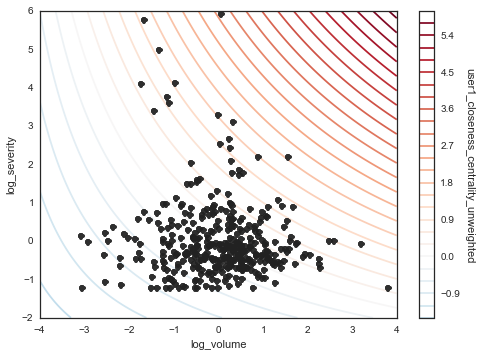
\includegraphics[width=\columnwidth]{centrality_volume_severity}
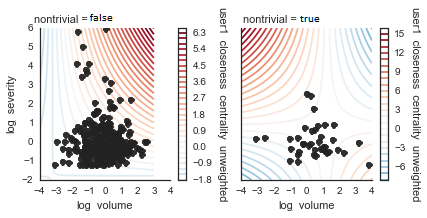
\includegraphics[width=\columnwidth]{centrality_volume_severity_nontrivial}
\end{figure}



\section{Future Work}
Our results suggest that bubble dynamics may be strongly influenced by founder effects, but that traditional network measures based on their position in the aggregate discussion graph do not provide a tight characterization of this effect.
As future work we are looking at coarse (positive/negative, detailed/cursory) semantic analysis of the discussion, and evidence of prior cooperation between pairs of participants in other altcoin markets, in order to attempt a more accurate characterization of core participants and their actions.

The features of the node as well as the construction of the graph are informed by a the pre-existing literature which does not allow for much complexity on the edges of the graphs beyond weight and direction.
A promising avenue for future work is to explore richer models for edges, in particular allowing them to exist in latent spaces, where he influence or attnetion that is payed by responding to a user is colored by the wording of the response. 
Two different avenues to learn such model suggest themselves: either using higher resolution time dynamics of the prices to learn to learn a space that captures the expectations implicitly forecasted by different language, or using NLP to attempt to parse these using other external corporate to know the multidimensional valence of the words.
%JULIAN: Seems a little too vague above
The cross-sectional design with time separation does not allow us to take advantage of intra-coin variation.
Beyond using data from forums, code repositories could also be exploited in future work as a rich source of variation beyond the binary feature of whether a coin is a trivial fork or not.


\section{Conclusion}
\section{Conclusion}


The total variance accounted for is small, so you need a discussion like "results suggest that bubble dynamics may be strongly influenced by a core set of participants, but that traditional network measures on the aggregate discussion graph do not provide a tight characterization of this core group.  We are looking at coarse (positive/negative, detailed/cursory) semantic analysis of the discussion, and evidence of prior cooperation between pairs of participants in other altcoin markets, in order to attempt this more accurate characterization of core participants and their actions.




% Table created by stargazer v.5.1 by Marek Hlavac, Harvard University. E-mail: hlavac at fas.harvard.edu
% Date and time: Mon, Jan 11, 2016 - 06:30:18
% Requires LaTeX packages: dcolumn 
\begin{table*}[!htbp] \centering 
  \caption{} 
  \label{} 
\begin{tabular}{@{\extracolsep{3pt}}lD{.}{.}{-3} D{.}{.}{-3} D{.}{.}{-3} D{.}{.}{-3} D{.}{.}{-3} } 
\\[-1.8ex]\hline 
\hline \\[-1.8ex] 
 & \multicolumn{5}{c}{Severity (BTC)} \\ 
\cline{2-6} 
\\[-1.8ex] & \multicolumn{5}{c}{} \\ 
 & \multicolumn{1}{c}{User} & \multicolumn{1}{c}{Satoshi} & \multicolumn{1}{c}{Network} & \multicolumn{1}{c}{Weighted} & \multicolumn{1}{c}{All} \\ 
\hline \\[-1.8ex] 
 Number of posts &  &  &  &  & -0.0002 \\ 
  &  &  &  &  & (0.0002) \\ 
  & & & & & \\ 
 Number of subjects & 0.007^{***} &  &  & 0.007^{***} & 0.008^{***} \\ 
  & (0.002) &  &  & (0.002) & (0.003) \\ 
  & & & & & \\ 
 Days since first post & -0.001^{***} &  &  & -0.001^{***} & -0.0005^{*} \\ 
  & (0.0002) &  &  & (0.0002) & (0.0003) \\ 
  & & & & & \\ 
 Incoming degree &  &  &  &  & -0.001 \\ 
  &  &  &  &  & (0.001) \\ 
  & & & & & \\ 
 Outgoing degree &  &  &  &  & 0.001 \\ 
  &  &  &  &  & (0.001) \\ 
  & & & & & \\ 
 Clustering coefficient &  &  &  &  & 0.148 \\ 
  &  &  &  &  & (1.003) \\ 
  & & & & & \\ 
 Closeness centrality &  &  & 0.017^{***} & 0.020^{***} & 0.019^{***} \\ 
  &  &  & (0.005) & (0.005) & (0.006) \\ 
  & & & & & \\ 
 Betweenness centrality &  &  &  &  & 0.00000 \\ 
  &  &  &  &  & (0.00000) \\ 
  & & & & & \\ 
 Satoshi distance &  & 0.135^{**} &  & 0.139^{**} & 0.176 \\ 
  &  & (0.062) &  & (0.065) & (0.108) \\ 
  & & & & & \\ 
 Infinite Satoshi distance &  &  &  &  & -0.384 \\ 
  &  &  &  &  & (0.467) \\ 
  & & & & & \\ 
 Satoshi pagerank &  &  &  &  & -1,027.712 \\ 
  &  &  &  &  & (685.442) \\ 
  & & & & & \\ 
 Pagerank &  &  &  &  & 524.431 \\ 
  &  &  &  &  & (421.395) \\ 
  & & & & & \\ 
 Coin Vintage Control & -0.002^{***} & -0.002^{***} & -0.001^{***} & -0.001^{***} & -0.001^{***} \\ 
  & (0.0002) & (0.0002) & (0.0003) & (0.0003) & (0.0003) \\ 
  & & & & & \\ 
 Constant & 2.494^{***} & 2.071^{***} & 0.996^{**} & 0.317 & 0.342 \\ 
  & (0.111) & (0.222) & (0.486) & (0.535) & (0.675) \\ 
  & & & & & \\ 
\hline \\[-1.8ex] 
Observations & \multicolumn{1}{c}{375} & \multicolumn{1}{c}{375} & \multicolumn{1}{c}{375} & \multicolumn{1}{c}{375} & \multicolumn{1}{c}{375} \\ 
R$^{2}$ & \multicolumn{1}{c}{0.187} & \multicolumn{1}{c}{0.176} & \multicolumn{1}{c}{0.206} & \multicolumn{1}{c}{0.240} & \multicolumn{1}{c}{0.247} \\ 
Adjusted R$^{2}$ & \multicolumn{1}{c}{0.180} & \multicolumn{1}{c}{0.172} & \multicolumn{1}{c}{0.202} & \multicolumn{1}{c}{0.229} & \multicolumn{1}{c}{0.220} \\ 
Residual Std. Error & \multicolumn{1}{c}{0.883} & \multicolumn{1}{c}{0.886} & \multicolumn{1}{c}{0.890} & \multicolumn{1}{c}{0.874} & \multicolumn{1}{c}{0.874} \\ 
F Statistic & \multicolumn{1}{c}{28.371$^{***}$} & \multicolumn{1}{c}{39.778$^{***}$} & \multicolumn{1}{c}{48.292$^{***}$} & \multicolumn{1}{c}{23.257$^{***}$} & \multicolumn{1}{c}{9.127$^{***}$} \\ 
\hline 
\hline \\[-1.8ex] 
\textit{Note:}  & \multicolumn{5}{r}{$^{*}$p$<$0.1; $^{**}$p$<$0.05; $^{***}$p$<$0.01} \\ 
\end{tabular} 
\end{table*} 

%\caption{Robust regression results of bubble severity as defined in variables section.
%Regression was performed using Huber weights after Elastic net feature selection. Empty
%cells indicate that the independent variable was not included in the model either
%explicitly or due to feature selection.}

% Table created by stargazer v.5.1 by Marek Hlavac, Harvard University. E-mail: hlavac at fas.harvard.edu
% Date and time: Mon, Jan 11, 2016 - 06:29:40
% Requires LaTeX packages: dcolumn 
\begin{table*}[!htbp] \centering 
  \caption{} 
  \label{} 
\begin{tabular}{@{\extracolsep{3pt}}lD{.}{.}{-3} D{.}{.}{-3} D{.}{.}{-3} D{.}{.}{-3} D{.}{.}{-3} } 
\\[-1.8ex]\hline 
\hline \\[-1.8ex] 
 & \multicolumn{5}{c}{Severity (USD)} \\ 
\cline{2-6} 
\\[-1.8ex] & \multicolumn{5}{c}{} \\ 
 & \multicolumn{1}{c}{Model1} & \multicolumn{1}{c}{Model2} & \multicolumn{1}{c}{Model3} & \multicolumn{1}{c}{Model4} & \multicolumn{1}{c}{Model5} \\ 
\hline \\[-1.8ex] 
 Number of posts & -0.0001 &  &  & -0.0001 & -0.0002 \\ 
  & (0.0001) &  &  & (0.0001) & (0.0002) \\ 
  & & & & & \\ 
 Number of subjects & 0.008^{***} &  &  & 0.008^{***} & 0.008^{***} \\ 
  & (0.003) &  &  & (0.003) & (0.003) \\ 
  & & & & & \\ 
 Days since first post & -0.0005^{**} &  &  & -0.0005^{**} & -0.0004 \\ 
  & (0.0002) &  &  & (0.0002) & (0.0003) \\ 
  & & & & & \\ 
 Incoming degree & -0.0001 &  &  &  & -0.0003 \\ 
  & (0.0003) &  &  &  & (0.001) \\ 
  & & & & & \\ 
 Outgoing degree &  &  &  &  & 0.0005 \\ 
  &  &  &  &  & (0.001) \\ 
  & & & & & \\ 
 Clustering coefficient &  &  &  &  & 0.504 \\ 
  &  &  &  &  & (0.995) \\ 
  & & & & & \\ 
 Closeness centrality &  &  & 0.013^{**} & 0.015^{***} & 0.014^{**} \\ 
  &  &  & (0.005) & (0.005) & (0.006) \\ 
  & & & & & \\ 
 Betweenness centrality &  &  & -0.000 &  & 0.00000 \\ 
  &  &  & (0.00000) &  & (0.00000) \\ 
  & & & & & \\ 
 Satoshi distance &  & 0.137^{**} &  & 0.130^{**} & 0.245^{**} \\ 
  &  & (0.062) &  & (0.064) & (0.107) \\ 
  & & & & & \\ 
 Infinite Satoshi distance &  &  &  &  & -0.711 \\ 
  &  &  &  &  & (0.465) \\ 
  & & & & & \\ 
 Satoshi pagerank &  &  &  &  & -630.044 \\ 
  &  &  &  &  & (681.502) \\ 
  & & & & & \\ 
 Pagerank &  &  &  &  & 419.387 \\ 
  &  &  &  &  & (418.583) \\ 
  & & & & & \\ 
 Coin Vintage Control & -0.002^{***} & -0.002^{***} & -0.002^{***} & -0.002^{***} & -0.002^{***} \\ 
  & (0.0002) & (0.0002) & (0.0003) & (0.0003) & (0.0003) \\ 
  & & & & & \\ 
 Constant & 2.911^{***} & 2.441^{***} & 1.720^{***} & 1.075^{**} & 0.789 \\ 
  & (0.130) & (0.220) & (0.477) & (0.527) & (0.667) \\ 
  & & & & & \\ 
\hline \\[-1.8ex] 
Observations & \multicolumn{1}{c}{375} & \multicolumn{1}{c}{375} & \multicolumn{1}{c}{375} & \multicolumn{1}{c}{375} & \multicolumn{1}{c}{375} \\ 
R$^{2}$ & \multicolumn{1}{c}{0.282} & \multicolumn{1}{c}{0.272} & \multicolumn{1}{c}{0.282} & \multicolumn{1}{c}{0.311} & \multicolumn{1}{c}{0.320} \\ 
Adjusted R$^{2}$ & \multicolumn{1}{c}{0.272} & \multicolumn{1}{c}{0.268} & \multicolumn{1}{c}{0.276} & \multicolumn{1}{c}{0.300} & \multicolumn{1}{c}{0.295} \\ 
Residual Std. Error & \multicolumn{1}{c}{0.895} & \multicolumn{1}{c}{0.892} & \multicolumn{1}{c}{0.886} & \multicolumn{1}{c}{0.873} & \multicolumn{1}{c}{0.871} \\ 
F Statistic & \multicolumn{1}{c}{28.974$^{***}$} & \multicolumn{1}{c}{69.382$^{***}$} & \multicolumn{1}{c}{48.530$^{***}$} & \multicolumn{1}{c}{27.694$^{***}$} & \multicolumn{1}{c}{13.043$^{***}$} \\ 
\hline 
\hline \\[-1.8ex] 
\textit{Note:}  & \multicolumn{5}{r}{$^{*}$p$<$0.1; $^{**}$p$<$0.05; $^{***}$p$<$0.01} \\ 
\end{tabular} 
\end{table*} 


%\caption{Robust regression results of bubble magnitude as defined in variables section.
%Regression was performed using Huber weights after Elastic net feature selection. Empty
%cells indicate that the independent variable was not included in the model either
%explicitly or due to feature selection. Note that train sample size is smaller than
%severity due to missing volume data in the first few trading days of several coins.}

% Table created by stargazer v.5.1 by Marek Hlavac, Harvard University. E-mail: hlavac at fas.harvard.edu
% Date and time: Mon, Jan 11, 2016 - 01:07:14
% Requires LaTeX packages: dcolumn 
\begin{table*}[!htbp] \centering 
  \caption{} 
  \label{} 
\begin{tabular}{@{\extracolsep{3pt}}lD{.}{.}{-3} D{.}{.}{-3} D{.}{.}{-3} D{.}{.}{-3} D{.}{.}{-3} } 
\\[-1.8ex]\hline 
\hline \\[-1.8ex] 
 & \multicolumn{5}{c}{Magnitude (USD)} \\ 
\cline{2-6} 
\\[-1.8ex] & \multicolumn{5}{c}{} \\ 
 & \multicolumn{1}{c}{Model1} & \multicolumn{1}{c}{Model2} & \multicolumn{1}{c}{Model3} & \multicolumn{1}{c}{Model4} & \multicolumn{1}{c}{Model5} \\ 
\hline \\[-1.8ex] 
 Number of posts &  &  &  &  & -0.0001 \\ 
  &  &  &  &  & (0.0002) \\ 
  & & & & & \\ 
 Number of subjects & 0.013^{***} &  &  & 0.013^{***} & 0.013^{***} \\ 
  & (0.003) &  &  & (0.003) & (0.003) \\ 
  & & & & & \\ 
 Days since first post & -0.001^{***} &  &  & -0.001^{***} & -0.001^{***} \\ 
  & (0.0004) &  &  & (0.0004) & (0.0004) \\ 
  & & & & & \\ 
 Incoming degree & 0.0005 &  &  &  & 0.003^{**} \\ 
  & (0.001) &  &  &  & (0.001) \\ 
  & & & & & \\ 
 Outgoing degree & -0.001 &  &  &  & 0.0002 \\ 
  & (0.001) &  &  &  & (0.002) \\ 
  & & & & & \\ 
 Clustering coefficient &  &  & -3.680^{**} & -2.915 & -1.671 \\ 
  &  &  & (1.787) & (1.812) & (1.919) \\ 
  & & & & & \\ 
 Closeness centrality &  &  &  &  & 0.059 \\ 
  &  &  &  &  & (0.150) \\ 
  & & & & & \\ 
 Betweenness centrality &  &  &  &  & -0.00000 \\ 
  &  &  &  &  & (0.00000) \\ 
  & & & & & \\ 
 Satoshi distance &  & -0.077 &  & -0.145 & -0.060 \\ 
  &  & (0.160) &  & (0.162) & (0.166) \\ 
  & & & & & \\ 
 Infinite Satoshi distance &  & -0.909 &  & -0.298 & -0.470 \\ 
  &  & (0.743) &  & (0.763) & (0.768) \\ 
  & & & & & \\ 
 Satoshi pagerank &  & -1,404.533^{*} &  & -1,209.802 & -1,827.999 \\ 
  &  & (739.320) &  & (817.544) & (2,188.413) \\ 
  & & & & & \\ 
 Pagerank &  &  &  &  & -674.396 \\ 
  &  &  &  &  & (978.634) \\ 
  & & & & & \\ 
 Coin Vintage Control & -0.002^{***} & -0.002^{***} & -0.002^{***} & -0.002^{***} & -0.002^{***} \\ 
  & (0.0004) & (0.0004) & (0.0004) & (0.0004) & (0.0004) \\ 
  & & & & & \\ 
 Constant & 2.584^{***} & 3.161^{***} & 2.778^{***} & 3.384^{***} & 2.829^{***} \\ 
  & (0.252) & (0.607) & (0.212) & (0.605) & (0.662) \\ 
  & & & & & \\ 
\hline \\[-1.8ex] 
Observations & \multicolumn{1}{c}{338} & \multicolumn{1}{c}{338} & \multicolumn{1}{c}{338} & \multicolumn{1}{c}{338} & \multicolumn{1}{c}{338} \\ 
R$^{2}$ & \multicolumn{1}{c}{0.161} & \multicolumn{1}{c}{0.132} & \multicolumn{1}{c}{0.121} & \multicolumn{1}{c}{0.181} & \multicolumn{1}{c}{0.195} \\ 
Adjusted R$^{2}$ & \multicolumn{1}{c}{0.149} & \multicolumn{1}{c}{0.121} & \multicolumn{1}{c}{0.115} & \multicolumn{1}{c}{0.164} & \multicolumn{1}{c}{0.162} \\ 
Residual Std. Error & \multicolumn{1}{c}{1.343} & \multicolumn{1}{c}{1.335} & \multicolumn{1}{c}{1.348} & \multicolumn{1}{c}{1.322} & \multicolumn{1}{c}{1.326} \\ 
F Statistic & \multicolumn{1}{c}{12.757$^{***}$} & \multicolumn{1}{c}{12.652$^{***}$} & \multicolumn{1}{c}{22.950$^{***}$} & \multicolumn{1}{c}{10.414$^{***}$} & \multicolumn{1}{c}{6.019$^{***}$} \\ 
\hline 
\hline \\[-1.8ex] 
\textit{Note:}  & \multicolumn{5}{r}{$^{*}$p$<$0.1; $^{**}$p$<$0.05; $^{***}$p$<$0.01} \\ 
\end{tabular} 
\end{table*} 


% Table created by stargazer v.5.1 by Marek Hlavac, Harvard University. E-mail: hlavac at fas.harvard.edu
% Date and time: Sun, Jan 10, 2016 - 04:22:04
% Requires LaTeX packages: dcolumn 
\begin{table*}[!htbp] \centering 
  \caption{} 
  \label{} 
\begin{tabular}{@{\extracolsep{3pt}}lD{.}{.}{-3} D{.}{.}{-3} D{.}{.}{-3} D{.}{.}{-3} D{.}{.}{-3} } 
\\[-1.8ex]\hline 
\hline \\[-1.8ex] 
 & \multicolumn{5}{c}{Magnitude (BTC)} \\ 
\cline{2-6} 
\\[-1.8ex] & \multicolumn{5}{c}{} \\ 
 & \multicolumn{1}{c}{Model1} & \multicolumn{1}{c}{Model2} & \multicolumn{1}{c}{Model3} & \multicolumn{1}{c}{Model4} & \multicolumn{1}{c}{Model5} \\ 
\hline \\[-1.8ex] 
 Number of posts &  &  &  &  & -0.0002 \\ 
  &  &  &  &  & (0.0003) \\ 
  & & & & & \\ 
 Number of subjects &  &  &  &  & 0.004 \\ 
  &  &  &  &  & (0.009) \\ 
  & & & & & \\ 
 Days since first post & -0.001^{***} &  &  & -0.001^{***} & -0.001^{***} \\ 
  & (0.0004) &  &  & (0.0004) & (0.0004) \\ 
  & & & & & \\ 
 Incoming degree & 0.001^{**} &  &  & 0.001^{*} & 0.003^{***} \\ 
  & (0.001) &  &  & (0.001) & (0.001) \\ 
  & & & & & \\ 
 Outgoing degree &  &  &  &  & 0.001 \\ 
  &  &  &  &  & (0.002) \\ 
  & & & & & \\ 
 Clustering coefficient &  &  & -2.479 &  & 0.758 \\ 
  &  &  & (2.182) &  & (2.428) \\ 
  & & & & & \\ 
 Closeness centrality &  &  & -179.899^{***} & -180.161^{***} & -109.986 \\ 
  &  &  & (68.190) & (61.738) & (76.436) \\ 
  & & & & & \\ 
 Betweenness centrality &  &  &  &  & -0.00000 \\ 
  &  &  &  &  & (0.00000) \\ 
  & & & & & \\ 
 Satoshi distance &  &  &  &  & 0.170 \\ 
  &  &  &  &  & (0.173) \\ 
  & & & & & \\ 
 Infinite Satoshi distance &  &  &  & -0.474 & -0.978 \\ 
  &  &  &  & (0.496) & (0.774) \\ 
  & & & & & \\ 
 Satoshi pagerank &  & -428.544 &  &  & 2,543.459 \\ 
  &  & (700.471) &  &  & (3,699.492) \\ 
  & & & & & \\ 
 Pagerank &  &  & -143.905 &  & -2,131.528 \\ 
  &  &  & (293.446) &  & (1,511.748) \\ 
  & & & & & \\ 
 Coin Vintage Control & -0.0004 &  & -0.002^{***} & -0.001^{**} & -0.001^{**} \\ 
  & (0.0004) &  & (0.0004) & (0.0004) & (0.0005) \\ 
  & & & & & \\ 
 Constant & 1.604^{***} & 1.343^{***} & 2.604^{***} & 2.294^{***} & 1.444^{*} \\ 
  & (0.251) & (0.091) & (0.328) & (0.341) & (0.755) \\ 
  & & & & & \\ 
\hline \\[-1.8ex] 
Observations & \multicolumn{1}{c}{339} & \multicolumn{1}{c}{339} & \multicolumn{1}{c}{339} & \multicolumn{1}{c}{339} & \multicolumn{1}{c}{339} \\ 
R$^{2}$ & \multicolumn{1}{c}{0.057} & \multicolumn{1}{c}{0.001} & \multicolumn{1}{c}{0.052} & \multicolumn{1}{c}{0.082} & \multicolumn{1}{c}{0.099} \\ 
Adjusted R$^{2}$ & \multicolumn{1}{c}{0.049} & \multicolumn{1}{c}{-0.002} & \multicolumn{1}{c}{0.041} & \multicolumn{1}{c}{0.068} & \multicolumn{1}{c}{0.063} \\ 
Residual Std. Error & \multicolumn{1}{c}{1.386} & \multicolumn{1}{c}{1.433} & \multicolumn{1}{c}{1.401} & \multicolumn{1}{c}{1.371} & \multicolumn{1}{c}{1.365} \\ 
F Statistic & \multicolumn{1}{c}{6.811$^{***}$} & \multicolumn{1}{c}{0.374} & \multicolumn{1}{c}{4.620$^{***}$} & \multicolumn{1}{c}{5.933$^{***}$} & \multicolumn{1}{c}{2.761$^{***}$} \\ 
\hline 
\hline \\[-1.8ex] 
\textit{Note:}  & \multicolumn{5}{r}{$^{*}$p$<$0.1; $^{**}$p$<$0.05; $^{***}$p$<$0.01} \\ 
\end{tabular} 
\end{table*} 



% Table created by stargazer v.5.1 by Marek Hlavac, Harvard University. E-mail: hlavac at fas.harvard.edu
% Date and time: Mon, Jan 11, 2016 - 01:46:11
% Requires LaTeX packages: dcolumn 
\begin{table*}[!htbp] \centering 
  \caption{} 
  \label{} 
\begin{tabular}{@{\extracolsep{0pt}}lD{.}{.}{-3} D{.}{.}{-3} D{.}{.}{-3} D{.}{.}{-3} D{.}{.}{-3} D{.}{.}{-3} D{.}{.}{-3} } 
\\[-1.8ex]\hline 
\hline \\[-1.8ex] 
 & \multicolumn{7}{c}{Severity (BTC)} \\ 
\cline{2-8} 
\\[-1.8ex] & \multicolumn{7}{c}{} \\ 
 & \multicolumn{1}{c}{Model2} & \multicolumn{1}{c}{Model3} & \multicolumn{1}{c}{Model4} & \multicolumn{1}{c}{Model5} & \multicolumn{1}{c}{Model6} & \multicolumn{1}{c}{Model7} & \multicolumn{1}{c}{Model8} \\ 
\hline \\[-1.8ex] 
 num posts &  &  &  &  &  &  & -0.0001 \\ 
  &  &  &  &  &  &  & (0.0002) \\ 
  num subjects &  &  &  &  & 0.007^{***} & 0.007^{***} & 0.007^{**} \\ 
  &  &  &  &  & (0.003) & (0.002) & (0.003) \\ 
  days since first post &  &  &  &  & -0.001^{***} & -0.001^{***} & -0.001^{**} \\ 
  &  &  &  &  & (0.0002) & (0.0002) & (0.0003) \\ 
  incoming degree &  &  &  &  &  &  & -0.001^{**} \\ 
  &  &  &  &  &  &  & (0.001) \\ 
  incoming * nontrivial &  &  &  &  &  &  & 0.006^{***} \\ 
  &  &  &  &  &  &  & (0.002) \\ 
  outgoing degree &  &  &  &  &  &  & 0.001 \\ 
  &  &  &  &  &  &  & (0.001) \\ 
  outgoing * nontrivial &  &  &  &  &  &  & 0.001 \\ 
  &  &  &  &  &  &  & (0.008) \\ 
  clustering coefficient &  &  & 1.123 &  & 1.425 &  & 0.939 \\ 
  &  &  & (0.868) &  & (0.873) &  & (0.942) \\ 
  clustering coefficient * nontrivial &  &  &  &  &  &  & 11.660 \\ 
  &  &  &  &  &  &  & (7.932) \\ 
  closeness centrality &  &  &  &  & -0.016 &  & -0.030 \\ 
  &  &  &  &  & (0.097) &  & (0.097) \\ 
  closeness * nontrivial &  &  &  &  &  &  & -51.947 \\ 
  &  &  &  &  &  &  & (89.808) \\ 
  betweenness centrality &  &  &  &  &  &  & 0.00000 \\ 
  &  &  &  &  &  &  & (0.00000) \\ 
  betweenness * nontrivial &  &  &  &  &  &  & 0.00000 \\ 
  &  &  &  &  &  &  & (0.00000) \\ 
  satoshi pagerank &  &  &  & -513.018 &  &  & 2,542.465 \\ 
  &  &  &  & (347.385) &  &  & (1,868.253) \\ 
  satoshi * nontrivial &  &  &  &  &  &  & -567.745 \\ 
  &  &  &  &  &  &  & (1,174.938) \\ 
  satoshi distance &  & 0.135^{**} &  &  &  &  & 0.169 \\ 
  &  & (0.062) &  &  &  &  & (0.109) \\ 
  Infinite satoshi distance &  &  &  &  &  &  & -0.551 \\ 
  &  &  &  &  &  &  & (0.479) \\ 
  pagerank &  &  &  &  &  &  & 836.085 \\ 
  &  &  &  &  &  &  & (512.426) \\ 
  pagerank * nontrivial &  &  &  &  &  &  & -3,080.895^{**} \\ 
  &  &  &  &  &  &  & (1,384.231) \\ 
  nontrivial & -0.042 &  &  &  &  &  & -0.597 \\ 
  & (0.173) &  &  &  &  &  & (0.387) \\ 
  Coin Vintage Control & -0.002^{***} & -0.002^{***} & -0.002^{***} & -0.002^{***} & -0.002^{***} & -0.002^{***} & -0.002^{***} \\ 
  & (0.0002) & (0.0002) & (0.0002) & (0.0002) & (0.0002) & (0.0002) & (0.0003) \\ 
  Constant & 2.520^{***} & 2.071^{***} & 2.449^{***} & 2.549^{***} & 2.435^{***} & 2.494^{***} & 1.882^{***} \\ 
  & (0.116) & (0.222) & (0.125) & (0.114) & (0.124) & (0.111) & (0.423) \\ 
 \hline \\[-1.8ex] 
Observations & \multicolumn{1}{c}{375} & \multicolumn{1}{c}{375} & \multicolumn{1}{c}{375} & \multicolumn{1}{c}{375} & \multicolumn{1}{c}{375} & \multicolumn{1}{c}{375} & \multicolumn{1}{c}{375} \\ 
R$^{2}$ & \multicolumn{1}{c}{0.167} & \multicolumn{1}{c}{0.176} & \multicolumn{1}{c}{0.173} & \multicolumn{1}{c}{0.173} & \multicolumn{1}{c}{0.194} & \multicolumn{1}{c}{0.187} & \multicolumn{1}{c}{0.250} \\ 
Adjusted R$^{2}$ & \multicolumn{1}{c}{0.163} & \multicolumn{1}{c}{0.172} & \multicolumn{1}{c}{0.169} & \multicolumn{1}{c}{0.169} & \multicolumn{1}{c}{0.184} & \multicolumn{1}{c}{0.180} & \multicolumn{1}{c}{0.206} \\ 
Residual Std. Error & \multicolumn{1}{c}{0.905} & \multicolumn{1}{c}{0.886} & \multicolumn{1}{c}{0.905} & \multicolumn{1}{c}{0.902} & \multicolumn{1}{c}{0.897} & \multicolumn{1}{c}{0.883} & \multicolumn{1}{c}{0.871} \\ 
F Statistic & \multicolumn{1}{c}{37.381$^{***}$} & \multicolumn{1}{c}{39.778$^{***}$} & \multicolumn{1}{c}{38.948$^{***}$} & \multicolumn{1}{c}{38.915$^{***}$} & \multicolumn{1}{c}{17.817$^{***}$} & \multicolumn{1}{c}{28.371$^{***}$} & \multicolumn{1}{c}{5.618$^{***}$} \\ 
\hline 
\hline \\[-1.8ex] 
\textit{Note:}  & \multicolumn{7}{r}{$^{*}$p$<$0.1; $^{**}$p$<$0.05; $^{***}$p$<$0.01} \\ 
\end{tabular} 
\end{table*} 

%\caption{Robust regression results of bubble severity as defined in variables section.
%Regression was performed using Huber weights after Elastic net feature selection. Empty
%cells indicate that the independent variable was not included in the model either
%explicitly or due to feature selection.}

% Table created by stargazer v.5.1 by Marek Hlavac, Harvard University. E-mail: hlavac at fas.harvard.edu
% Date and time: Mon, Jan 11, 2016 - 06:43:42
% Requires LaTeX packages: dcolumn 
\begin{table*}[!htbp] \centering 
  \caption{} 
  \label{} 
\begin{tabular}{@{\extracolsep{0pt}}lD{.}{.}{-3} D{.}{.}{-3} D{.}{.}{-3} D{.}{.}{-3} D{.}{.}{-3} D{.}{.}{-3} D{.}{.}{-3} } 
\\[-1.8ex]\hline 
\hline \\[-1.8ex] 
 & \multicolumn{7}{c}{Severity (USD)} \\ 
\cline{2-8} 
\\[-1.8ex] & \multicolumn{7}{c}{} \\ 
 & \multicolumn{1}{c}{Model2} & \multicolumn{1}{c}{Model3} & \multicolumn{1}{c}{Model4} & \multicolumn{1}{c}{Model5} & \multicolumn{1}{c}{Model6} & \multicolumn{1}{c}{Model7} & \multicolumn{1}{c}{Model8} \\ 
\hline \\[-1.8ex] 
 num posts &  &  &  &  & -0.0001 &  & -0.0002 \\ 
  &  &  &  &  & (0.0001) &  & (0.0002) \\ 
  num subjects &  &  &  &  & 0.008^{***} & 0.007^{***} & 0.008^{***} \\ 
  &  &  &  &  & (0.003) & (0.002) & (0.003) \\ 
  days since first post &  &  &  &  & -0.0005^{**} & -0.001^{***} & -0.001^{**} \\ 
  &  &  &  &  & (0.0002) & (0.0002) & (0.0003) \\ 
  incoming degree &  &  &  &  &  &  & -0.001 \\ 
  &  &  &  &  &  &  & (0.001) \\ 
  incoming * nontrivial &  &  &  &  &  & 0.0005 & 0.006^{***} \\ 
  &  &  &  &  &  & (0.001) & (0.002) \\ 
  outgoing degree &  &  &  &  &  &  & 0.001 \\ 
  &  &  &  &  &  &  & (0.001) \\ 
  outgoing * nontrivial &  &  &  &  &  &  & -0.0001 \\ 
  &  &  &  &  &  &  & (0.008) \\ 
  clustering coefficient &  &  &  &  &  &  & 0.389 \\ 
  &  &  &  &  &  &  & (0.984) \\ 
  clustering coefficient * nontrivial &  &  &  &  &  &  & 16.910^{**} \\ 
  &  &  &  &  &  &  & (7.970) \\ 
  closeness centrality &  &  & 0.013^{**} &  & 0.015^{***} & 0.016^{***} & 0.014^{**} \\ 
  &  &  & (0.005) &  & (0.005) & (0.005) & (0.007) \\ 
  closeness * nontrivial &  &  &  &  &  &  & -0.024 \\ 
  &  &  &  &  &  &  & (0.019) \\ 
  betweenness centrality &  &  & -0.000 &  &  &  & 0.00000 \\ 
  &  &  & (0.00000) &  &  &  & (0.00000) \\ 
  betweenness * nontrivial &  &  &  &  &  & 0.00000 & 0.00000 \\ 
  &  &  &  &  &  & (0.00000) & (0.00000) \\ 
  satoshi pagerank &  &  &  &  &  &  & -593.697 \\ 
  &  &  &  &  &  &  & (1,095.221) \\ 
  satoshi * nontrivial &  &  &  &  &  &  & 3,052.589^{*} \\ 
  &  &  &  &  &  &  & (1,769.639) \\ 
  satoshi distance &  & 0.137^{**} &  &  & 0.130^{**} &  & 0.239^{**} \\ 
  &  & (0.062) &  &  & (0.064) &  & (0.106) \\ 
  Infinite satoshi distance &  &  &  &  &  &  & -0.842^{*} \\ 
  &  &  &  &  &  &  & (0.468) \\ 
  pagerank &  &  &  &  &  &  & 529.551 \\ 
  &  &  &  &  &  &  & (508.684) \\ 
  pagerank * nontrivial &  &  &  &  &  &  & -3,181.144^{**} \\ 
  &  &  &  &  &  &  & (1,281.422) \\ 
  nontrivial & 0.058 &  &  &  &  &  & 0.806 \\ 
  & (0.172) &  &  &  &  &  & (1.196) \\ 
  Coin Vintage Control & -0.002^{***} & -0.002^{***} & -0.002^{***} & -0.002^{***} & -0.002^{***} & -0.001^{***} & -0.002^{***} \\ 
  & (0.0002) & (0.0002) & (0.0003) & (0.0002) & (0.0003) & (0.0003) & (0.0003) \\ 
  Constant & 2.858^{***} & 2.441^{***} & 1.720^{***} & 2.868^{***} & 1.075^{**} & 1.415^{***} & 0.841 \\ 
  & (0.113) & (0.220) & (0.477) & (0.109) & (0.527) & (0.478) & (0.681) \\ 
 \hline \\[-1.8ex] 
Observations & \multicolumn{1}{c}{375} & \multicolumn{1}{c}{375} & \multicolumn{1}{c}{375} & \multicolumn{1}{c}{375} & \multicolumn{1}{c}{375} & \multicolumn{1}{c}{375} & \multicolumn{1}{c}{375} \\ 
R$^{2}$ & \multicolumn{1}{c}{0.263} & \multicolumn{1}{c}{0.272} & \multicolumn{1}{c}{0.282} & \multicolumn{1}{c}{0.263} & \multicolumn{1}{c}{0.311} & \multicolumn{1}{c}{0.311} & \multicolumn{1}{c}{0.355} \\ 
Adjusted R$^{2}$ & \multicolumn{1}{c}{0.259} & \multicolumn{1}{c}{0.268} & \multicolumn{1}{c}{0.276} & \multicolumn{1}{c}{0.261} & \multicolumn{1}{c}{0.300} & \multicolumn{1}{c}{0.299} & \multicolumn{1}{c}{0.316} \\ 
Residual Std. Error & \multicolumn{1}{c}{0.897} & \multicolumn{1}{c}{0.892} & \multicolumn{1}{c}{0.886} & \multicolumn{1}{c}{0.896} & \multicolumn{1}{c}{0.873} & \multicolumn{1}{c}{0.878} & \multicolumn{1}{c}{0.854} \\ 
F Statistic & \multicolumn{1}{c}{66.506$^{***}$} & \multicolumn{1}{c}{69.382$^{***}$} & \multicolumn{1}{c}{48.530$^{***}$} & \multicolumn{1}{c}{133.172$^{***}$} & \multicolumn{1}{c}{27.694$^{***}$} & \multicolumn{1}{c}{27.630$^{***}$} & \multicolumn{1}{c}{9.242$^{***}$} \\ 
\hline 
\hline \\[-1.8ex] 
\textit{Note:}  & \multicolumn{7}{r}{$^{*}$p$<$0.1; $^{**}$p$<$0.05; $^{***}$p$<$0.01} \\ 
\end{tabular} 
\end{table*} 


%\caption{Robust regression results of bubble magnitude as defined in variables section.
%Regression was performed using Huber weights after Elastic net feature selection. Empty
%cells indicate that the independent variable was not included in the model either
%explicitly or due to feature selection. Note that train sample size is smaller than
%severity due to missing volume data in the first few trading days of several coins.}

% Table created by stargazer v.5.1 by Marek Hlavac, Harvard University. E-mail: hlavac at fas.harvard.edu
% Date and time: Mon, Jan 11, 2016 - 06:43:14
% Requires LaTeX packages: dcolumn 
\begin{table*}[!htbp] \centering 
  \caption{} 
  \label{} 
\begin{tabular}{@{\extracolsep{0pt}}lD{.}{.}{-3} D{.}{.}{-3} D{.}{.}{-3} D{.}{.}{-3} D{.}{.}{-3} D{.}{.}{-3} D{.}{.}{-3} } 
\\[-1.8ex]\hline 
\hline \\[-1.8ex] 
 & \multicolumn{7}{c}{Magnitude (USD)} \\ 
\cline{2-8} 
\\[-1.8ex] & \multicolumn{7}{c}{} \\ 
 & \multicolumn{1}{c}{Model2} & \multicolumn{1}{c}{Model3} & \multicolumn{1}{c}{Model4} & \multicolumn{1}{c}{Model5} & \multicolumn{1}{c}{Model6} & \multicolumn{1}{c}{Model7} & \multicolumn{1}{c}{Model8} \\ 
\hline \\[-1.8ex] 
 num posts &  &  &  &  &  &  & -0.0001 \\ 
  &  &  &  &  &  &  & (0.0002) \\ 
  num subjects &  &  &  &  &  &  & 0.002 \\ 
  &  &  &  &  &  &  & (0.002) \\ 
  days since first post &  &  &  &  & -0.0003 & -0.0003 & -0.001^{*} \\ 
  &  &  &  &  & (0.0002) & (0.0002) & (0.0003) \\ 
  incoming degree &  &  &  &  &  &  & -0.001^{*} \\ 
  &  &  &  &  &  &  & (0.001) \\ 
  incoming * nontrivial &  &  &  &  &  &  & 0.009^{***} \\ 
  &  &  &  &  &  &  & (0.003) \\ 
  outgoing degree &  &  &  &  &  &  & 0.0001 \\ 
  &  &  &  &  &  &  & (0.001) \\ 
  outgoing * nontrivial &  &  &  &  &  &  & -0.002 \\ 
  &  &  &  &  &  &  & (0.015) \\ 
  clustering coefficient &  &  & 0.181 &  &  &  & -0.058 \\ 
  &  &  & (1.226) &  &  &  & (1.302) \\ 
  clustering coefficient * nontrivial &  &  &  &  &  &  & 18.067 \\ 
  &  &  &  &  &  &  & (14.267) \\ 
  closeness centrality &  &  & -0.008 &  &  &  & -0.013 \\ 
  &  &  & (0.011) &  &  &  & (0.012) \\ 
  closeness * nontrivial &  &  &  &  &  &  & 0.002 \\ 
  &  &  &  &  &  &  & (0.037) \\ 
  betweenness centrality &  &  & -0.000 &  &  &  & 0.00000 \\ 
  &  &  & (0.000) &  &  &  & (0.00000) \\ 
  betweenness * nontrivial &  &  &  &  &  &  & -0.00000 \\ 
  &  &  &  &  &  &  & (0.00000) \\ 
  satoshi pagerank &  &  &  &  &  &  & -107.981 \\ 
  &  &  &  &  &  &  & (2,021.106) \\ 
  satoshi * nontrivial &  &  &  &  &  &  & -7,843.748 \\ 
  &  &  &  &  &  &  & (7,218.118) \\ 
  satoshi distance &  &  &  &  &  &  & 0.027 \\ 
  &  &  &  &  &  &  & (0.113) \\ 
  Infinite satoshi distance &  &  &  &  &  &  & -0.257 \\ 
  &  &  &  &  &  &  & (0.499) \\ 
  pagerank &  &  & 314.318 &  &  &  & 899.859 \\ 
  &  &  & (216.038) &  &  &  & (812.427) \\ 
  pagerank * nontrivial &  &  &  &  &  &  & -54.428 \\ 
  &  &  &  &  &  &  & (2,286.421) \\ 
  nontrivial & -0.149 &  &  &  &  &  & -1.492 \\ 
  & (0.192) &  &  &  &  &  & (2.517) \\ 
  Coin Vintage Control & -0.002^{***} & -0.002^{***} & -0.002^{***} & -0.002^{***} & -0.002^{***} & -0.002^{***} & -0.002^{***} \\ 
  & (0.0002) & (0.0002) & (0.0003) & (0.0002) & (0.0002) & (0.0002) & (0.0003) \\ 
  Constant & 2.698^{***} & 2.674^{***} & 3.132^{***} & 2.674^{***} & 2.660^{***} & 2.660^{***} & 3.579^{***} \\ 
  & (0.143) & (0.140) & (0.847) & (0.140) & (0.139) & (0.139) & (1.076) \\ 
 \hline \\[-1.8ex] 
Observations & \multicolumn{1}{c}{339} & \multicolumn{1}{c}{339} & \multicolumn{1}{c}{339} & \multicolumn{1}{c}{339} & \multicolumn{1}{c}{339} & \multicolumn{1}{c}{339} & \multicolumn{1}{c}{339} \\ 
R$^{2}$ & \multicolumn{1}{c}{0.162} & \multicolumn{1}{c}{0.159} & \multicolumn{1}{c}{0.168} & \multicolumn{1}{c}{0.159} & \multicolumn{1}{c}{0.163} & \multicolumn{1}{c}{0.163} & \multicolumn{1}{c}{0.213} \\ 
Adjusted R$^{2}$ & \multicolumn{1}{c}{0.157} & \multicolumn{1}{c}{0.157} & \multicolumn{1}{c}{0.155} & \multicolumn{1}{c}{0.157} & \multicolumn{1}{c}{0.158} & \multicolumn{1}{c}{0.158} & \multicolumn{1}{c}{0.161} \\ 
Residual Std. Error & \multicolumn{1}{c}{0.898} & \multicolumn{1}{c}{0.898} & \multicolumn{1}{c}{0.894} & \multicolumn{1}{c}{0.898} & \multicolumn{1}{c}{0.891} & \multicolumn{1}{c}{0.891} & \multicolumn{1}{c}{0.887} \\ 
F Statistic & \multicolumn{1}{c}{32.405$^{***}$} & \multicolumn{1}{c}{63.937$^{***}$} & \multicolumn{1}{c}{13.420$^{***}$} & \multicolumn{1}{c}{63.937$^{***}$} & \multicolumn{1}{c}{32.686$^{***}$} & \multicolumn{1}{c}{32.686$^{***}$} & \multicolumn{1}{c}{4.080$^{***}$} \\ 
\hline 
\hline \\[-1.8ex] 
\textit{Note:}  & \multicolumn{7}{r}{$^{*}$p$<$0.1; $^{**}$p$<$0.05; $^{***}$p$<$0.01} \\ 
\end{tabular} 
\end{table*} 


% Table created by stargazer v.5.1 by Marek Hlavac, Harvard University. E-mail: hlavac at fas.harvard.edu
% Date and time: Mon, Jan 11, 2016 - 01:44:30
% Requires LaTeX packages: dcolumn 
\begin{table*}[!htbp] \centering 
  \caption{} 
  \label{} 
\begin{tabular}{@{\extracolsep{0pt}}lD{.}{.}{-3} D{.}{.}{-3} D{.}{.}{-3} D{.}{.}{-3} D{.}{.}{-3} D{.}{.}{-3} D{.}{.}{-3} } 
\\[-1.8ex]\hline 
\hline \\[-1.8ex] 
 & \multicolumn{7}{c}{Magnitude (BTC)} \\ 
\cline{2-8} 
\\[-1.8ex] & \multicolumn{7}{c}{} \\ 
 & \multicolumn{1}{c}{Model2} & \multicolumn{1}{c}{Model3} & \multicolumn{1}{c}{Model4} & \multicolumn{1}{c}{Model5} & \multicolumn{1}{c}{Model6} & \multicolumn{1}{c}{Model7} & \multicolumn{1}{c}{Model8} \\ 
\hline \\[-1.8ex] 
 num posts &  &  &  &  &  &  & 0.0003 \\ 
  &  &  &  &  &  &  & (0.0003) \\ 
  num subjects &  &  &  &  &  &  & 0.005^{***} \\ 
  &  &  &  &  &  &  & (0.002) \\ 
  days since first post &  &  &  &  & -0.0002 &  & -0.0004 \\ 
  &  &  &  &  & (0.0002) &  & (0.0003) \\ 
  incoming degree &  &  &  &  &  &  & -0.001^{*} \\ 
  &  &  &  &  &  &  & (0.001) \\ 
  incoming * nontrivial &  &  &  &  &  &  & 0.003 \\ 
  &  &  &  &  &  &  & (0.003) \\ 
  outgoing degree &  &  &  &  &  &  & -0.001 \\ 
  &  &  &  &  &  &  & (0.002) \\ 
  outgoing * nontrivial &  &  &  &  &  &  & 0.007 \\ 
  &  &  &  &  &  &  & (0.013) \\ 
  clustering coefficient &  &  &  &  &  &  & 0.131 \\ 
  &  &  &  &  &  &  & (1.513) \\ 
  clustering coefficient * nontrivial &  &  &  &  &  &  & -3.209 \\ 
  &  &  &  &  &  &  & (14.580) \\ 
  closeness centrality &  &  &  &  &  &  & -0.041 \\ 
  &  &  &  &  &  &  & (0.103) \\ 
  closeness * nontrivial &  &  &  &  &  &  & -90.775 \\ 
  &  &  &  &  &  &  & (152.582) \\ 
  betweenness centrality &  &  &  &  &  &  & 0.000 \\ 
  &  &  &  &  &  &  & (0.00000) \\ 
  betweenness * nontrivial &  &  &  &  &  &  & -0.00000 \\ 
  &  &  &  &  &  &  & (0.00000) \\ 
  satoshi pagerank &  & 807.645 &  &  &  &  & -223.809 \\ 
  &  & (502.113) &  &  &  &  & (1,541.629) \\ 
  satoshi * nontrivial &  &  &  &  &  &  & -13,058.490 \\ 
  &  &  &  &  &  &  & (8,051.614) \\ 
  satoshi distance &  & 0.227^{**} &  &  &  &  & 0.166 \\ 
  &  & (0.101) &  &  &  &  & (0.107) \\ 
  Infinite satoshi distance &  & -0.938^{**} &  &  &  &  & -0.799^{*} \\ 
  &  & (0.423) &  &  &  &  & (0.439) \\ 
  pagerank &  &  &  &  &  &  & 805.888 \\ 
  &  &  &  &  &  &  & (658.294) \\ 
  pagerank * nontrivial &  &  &  &  &  &  & 6,715.020 \\ 
  &  &  &  &  &  &  & (4,315.273) \\ 
  nontrivial & -0.120 &  &  &  &  &  & -0.719 \\ 
  & (0.178) &  &  &  &  &  & (0.451) \\ 
  Coin Vintage Control & -0.001^{***} & -0.001^{***} & -0.001^{***} & -0.001^{***} & -0.001^{***} & -0.001^{***} & -0.001^{***} \\ 
  & (0.0002) & (0.0002) & (0.0002) & (0.0002) & (0.0002) & (0.0002) & (0.0003) \\ 
  Constant & 2.160^{***} & 1.286^{***} & 2.134^{***} & 2.134^{***} & 2.124^{***} & 2.134^{***} & 1.547^{***} \\ 
  & (0.141) & (0.394) & (0.137) & (0.137) & (0.136) & (0.137) & (0.447) \\ 
 \hline \\[-1.8ex] 
Observations & \multicolumn{1}{c}{338} & \multicolumn{1}{c}{338} & \multicolumn{1}{c}{338} & \multicolumn{1}{c}{338} & \multicolumn{1}{c}{338} & \multicolumn{1}{c}{338} & \multicolumn{1}{c}{338} \\ 
R$^{2}$ & \multicolumn{1}{c}{0.070} & \multicolumn{1}{c}{0.088} & \multicolumn{1}{c}{0.069} & \multicolumn{1}{c}{0.069} & \multicolumn{1}{c}{0.072} & \multicolumn{1}{c}{0.069} & \multicolumn{1}{c}{0.160} \\ 
Adjusted R$^{2}$ & \multicolumn{1}{c}{0.065} & \multicolumn{1}{c}{0.077} & \multicolumn{1}{c}{0.066} & \multicolumn{1}{c}{0.066} & \multicolumn{1}{c}{0.066} & \multicolumn{1}{c}{0.066} & \multicolumn{1}{c}{0.104} \\ 
Residual Std. Error & \multicolumn{1}{c}{0.852} & \multicolumn{1}{c}{0.846} & \multicolumn{1}{c}{0.850} & \multicolumn{1}{c}{0.850} & \multicolumn{1}{c}{0.845} & \multicolumn{1}{c}{0.850} & \multicolumn{1}{c}{0.821} \\ 
F Statistic & \multicolumn{1}{c}{12.638$^{***}$} & \multicolumn{1}{c}{7.999$^{***}$} & \multicolumn{1}{c}{24.897$^{***}$} & \multicolumn{1}{c}{24.897$^{***}$} & \multicolumn{1}{c}{12.909$^{***}$} & \multicolumn{1}{c}{24.897$^{***}$} & \multicolumn{1}{c}{2.857$^{***}$} \\ 
\hline 
\hline \\[-1.8ex] 
\textit{Note:}  & \multicolumn{7}{r}{$^{*}$p$<$0.1; $^{**}$p$<$0.05; $^{***}$p$<$0.01} \\ 
\end{tabular} 
\end{table*} 


%\section{Acknowledgments}

% You must have a proper ".bib" file
%  and remember to run:
% latex bibtex latex latex
% to resolve all references
\bibliography{references}
\bibliographystyle{aaai}


\end{document}


